\documentclass[10pt, a4paper]{beamer}
\usepackage{graphicx}
\usetheme{Berkeley}
\usecolortheme{sidebartab}

\begin{document}
	\setbeamertemplate{sidebar left}{}
	\title{Progress Presentation-I}
	\subtitle{e-Yantra Summer Intership-2016 \\ $Sign-Language Interpreter (Leap Motion Sensor)$}
	\author{Sanket R Bhimani\\
	Mentor: Rama sir \& Aditya sir}
	\institute{IIT Bombay}
	\date{\today}
	%\addtobeamertemplate{sidebar left}{}{\includegraphics[scale = 0.3]{logowithtext.png}}
	\frame{\titlepage}

\setbeamertemplate{sidebar left}[sidebar theme]
\section{Overview of Project}
\begin{frame}{Overview of Project}
\vspace{-45px}
\center{\huge{Sign-Language Interpreter \\(Leap Motion Sensor)}}
\vspace{15px}
	\begin{itemize}
		\item Objective
		\begin{itemize}
		    \item This project aims to help deaf and dumb people to communicate with normal person who are not aware of sign language.
		\end{itemize}
		\item Deliverable
		\begin{itemize}
		    \item Map words with pre-recorded speech.
		    \item Design Tutorial and Documentation of project with video demonstration.
		\end{itemize}
	\end{itemize}
\end{frame}

\section{Overview of Task}
\begin{frame}{Overview of Task}
\hspace{-21px}
\begin{tabular}{c|c|c}
    \hline
    Task No.&Task&Deadline\\
    \hline
    1&Get Familiar with Leap Motion Sensor&\\& and Galileo Board&3 days\\
    \hline
    2&Interfacing and Testing of Leap Motion Sensor.&\\
    &Generation of data for&\\& different hands/fingers used&2 days\\
    \hline
    3&Individual hand gesture for the alphabets &\\&should be recorded&3 days\\
    \hline
    4&Record gesture for words and calibration of &\\&leap motion sensor for sign language recognition&3 days\\
    \hline
    5&Communication the data between Leap  &\\&Motion Sensor and Galileo  board via local network&1 days\\
    \hline
    6&Interface mp3 module with  Galileo Board and&\\& map recognized words to pre-recorded  speech.&4 days\\
    \hline
    7&Design Tutorial and Documentation of&\\& project with video demonstration.&5 days\\
\end{tabular}
\end{frame}

\section{Task Accomplished}
\begin{frame}{Task Accomplished}
	\begin{itemize}
		\item Task 1 (Get familiar with sensor and board)
		\begin{itemize}
		    \item In this task Linux was installed on Galileo board and run some basic programme on board.
		    \item Seen stuff in Leap Motion Control Panel and see applications there.
		    \item Search about how to develop with Leap Motion Sensor and found Leap SDK.
		\end{itemize}
		\item Task 2 (Generation of data for different hands and fingers)
		\begin{itemize}
		    \item In this task I have studied about Leap SDK and it's Library 
		    \item And make simple programme for displaying  data related position and direction of hands and fingers
		\end{itemize}
	\end{itemize}
\end{frame}
\section{Task Accomplished}
\begin{frame}{Task Accomplished}
    \begin{itemize}
        \item Task 3 (Individual alphabet recognize)
		\begin{itemize}
		    \item In this task one programme is made in which we need to first load pose with one alphabet and then we can recognize that alphabet by performing that pose
		\end{itemize}
		\item Task 4 (Record gesture for words)
		\begin{itemize}
		    \item Here one interface is used for recording and recognizing gesture for particular word or sentence.
		\end{itemize}
		\item Task 5 (Communication between Leap and Galileo Board)
		\begin{itemize}
		    \item Here Websocket on localnetwork is used to transmit data between Leap and Galileo. 
		\end{itemize}
	\end{itemize}
\end{frame}
\section{Task Accomplished}
\begin{frame}{Task Accomplished}
    \center{\Large{Task 4 (Record gesture for words)}}
	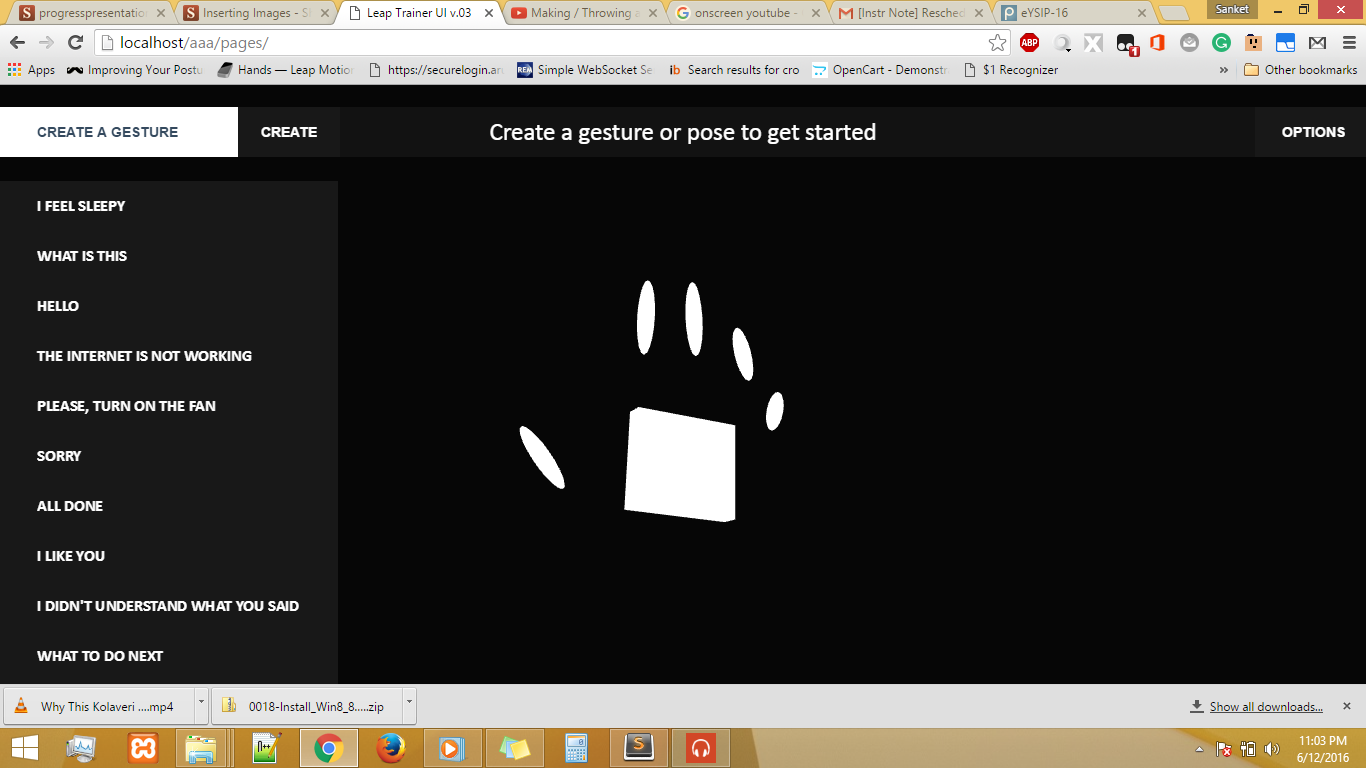
\includegraphics[totalheight=0.75\textheight]{ui}
\end{frame}
\section{Task Accomplished}
\begin{frame}{Task Accomplished}
	\center{\Large{Task 4 (Record gesture for words)}}
	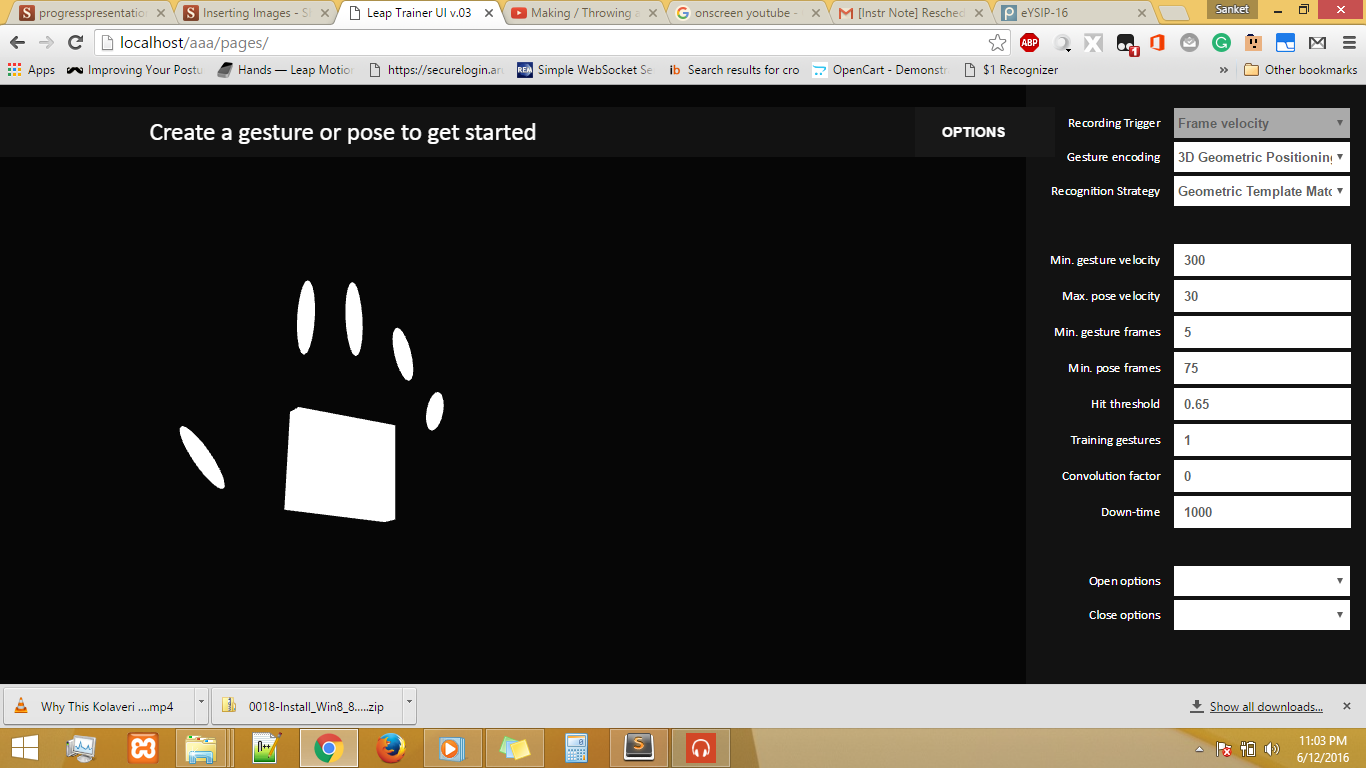
\includegraphics[totalheight=0.75\textheight]{ui_options}
\end{frame}
\section{Challenges Faced}
\begin{frame}{Challenges Faced}
	\begin{itemize}
		\item Recording and Recognizing Gestures in Leap motion Sensor
		\item Installing Windows IOT on Galileo
		\item Making sentence from basic words generated from system
	\end{itemize}
\end{frame}

\section{Future Plans}
\begin{frame}{Future Plans}
	\begin{itemize}
		\item Interfacing with MP3 module is remaining in my task
		\item Making sentence generation more reliable
		\item Load more words and make system more accurate..
		\item Making robotics hand which will be operated by moving our hand. 
	\end{itemize}
\end{frame}


\section{Thank You}
\begin{frame}{Thank You}
	\centering THANK YOU !!!
\end{frame}
\end{document}
